% !TEX root = main.tex
\chapter{Aerodynamic Effects on Vehicle Performance}

  Understanding the theoretical background as to why aerodynamics is important for a vehicles's handling requires knowledge of how a vehicle's top speed and cornering performance depends on drag, grip and how downforce differs from mass. The first theoretical segment covers how top speed changes with aerodynamics on straights and during cornering, in order to understand the behaviour of a racing vehicle.

\section{Drag Effects on Straights}
\label{sec:topspeed}

  First, let's explain what makes a car fast, and what parameters we can change to improve the speed of our car. The car's acceleration can be described by Newton's second law as:\fxnote{stort D eller lille d i ligningen?}
  \begin{align}
    \sum F_x &= m \ddot{x} = F
    \intertext{Where the sum of forces in the x-direction (the direction of travel) can be expressed as the force already pertained by the vehicle, minus the drag force:}
    F &- C_D \left(\frac{1}{2}  \rho \dot{x}^2 A \right) = m \ddot{x}
    \intertext{Where $C_D$ is the drag coefficient of the vehicle, $\rho$ is the density of the fluid it moves in and $A$ is frontal area of the vehicle. Assuming we're moving at a steady speed, the acceleration is 0, hence}
    F &= C_D \left(\frac{1}{2}  \rho \dot{x}^2 A \right)
    \intertext{As we were interested in the speed of the car, let's solve for the velocity. The force is given by $F = \frac{P}{\dot{x}}$, where $P$ is the power of the car, which gives:}
    \dot{x} &= \left( \frac{2 P}{C_D \left(\rho A \right)}\right)^{\frac{1}{3}}
  \end{align}
  This is assuming we're traveling at terminal velocity -- that is, the point where the $\text{Driving Force} = \text{Friction Force}$. The terminal velocity of the racer is then easily calculated, as the competition restricts the maximum amount of power to $\SI{80}{\kilo\watt}$, and the frontal area of the car is approximated from the CAD drawing seen in figure \ref{fig:frontarea}

  \begin{figure}
    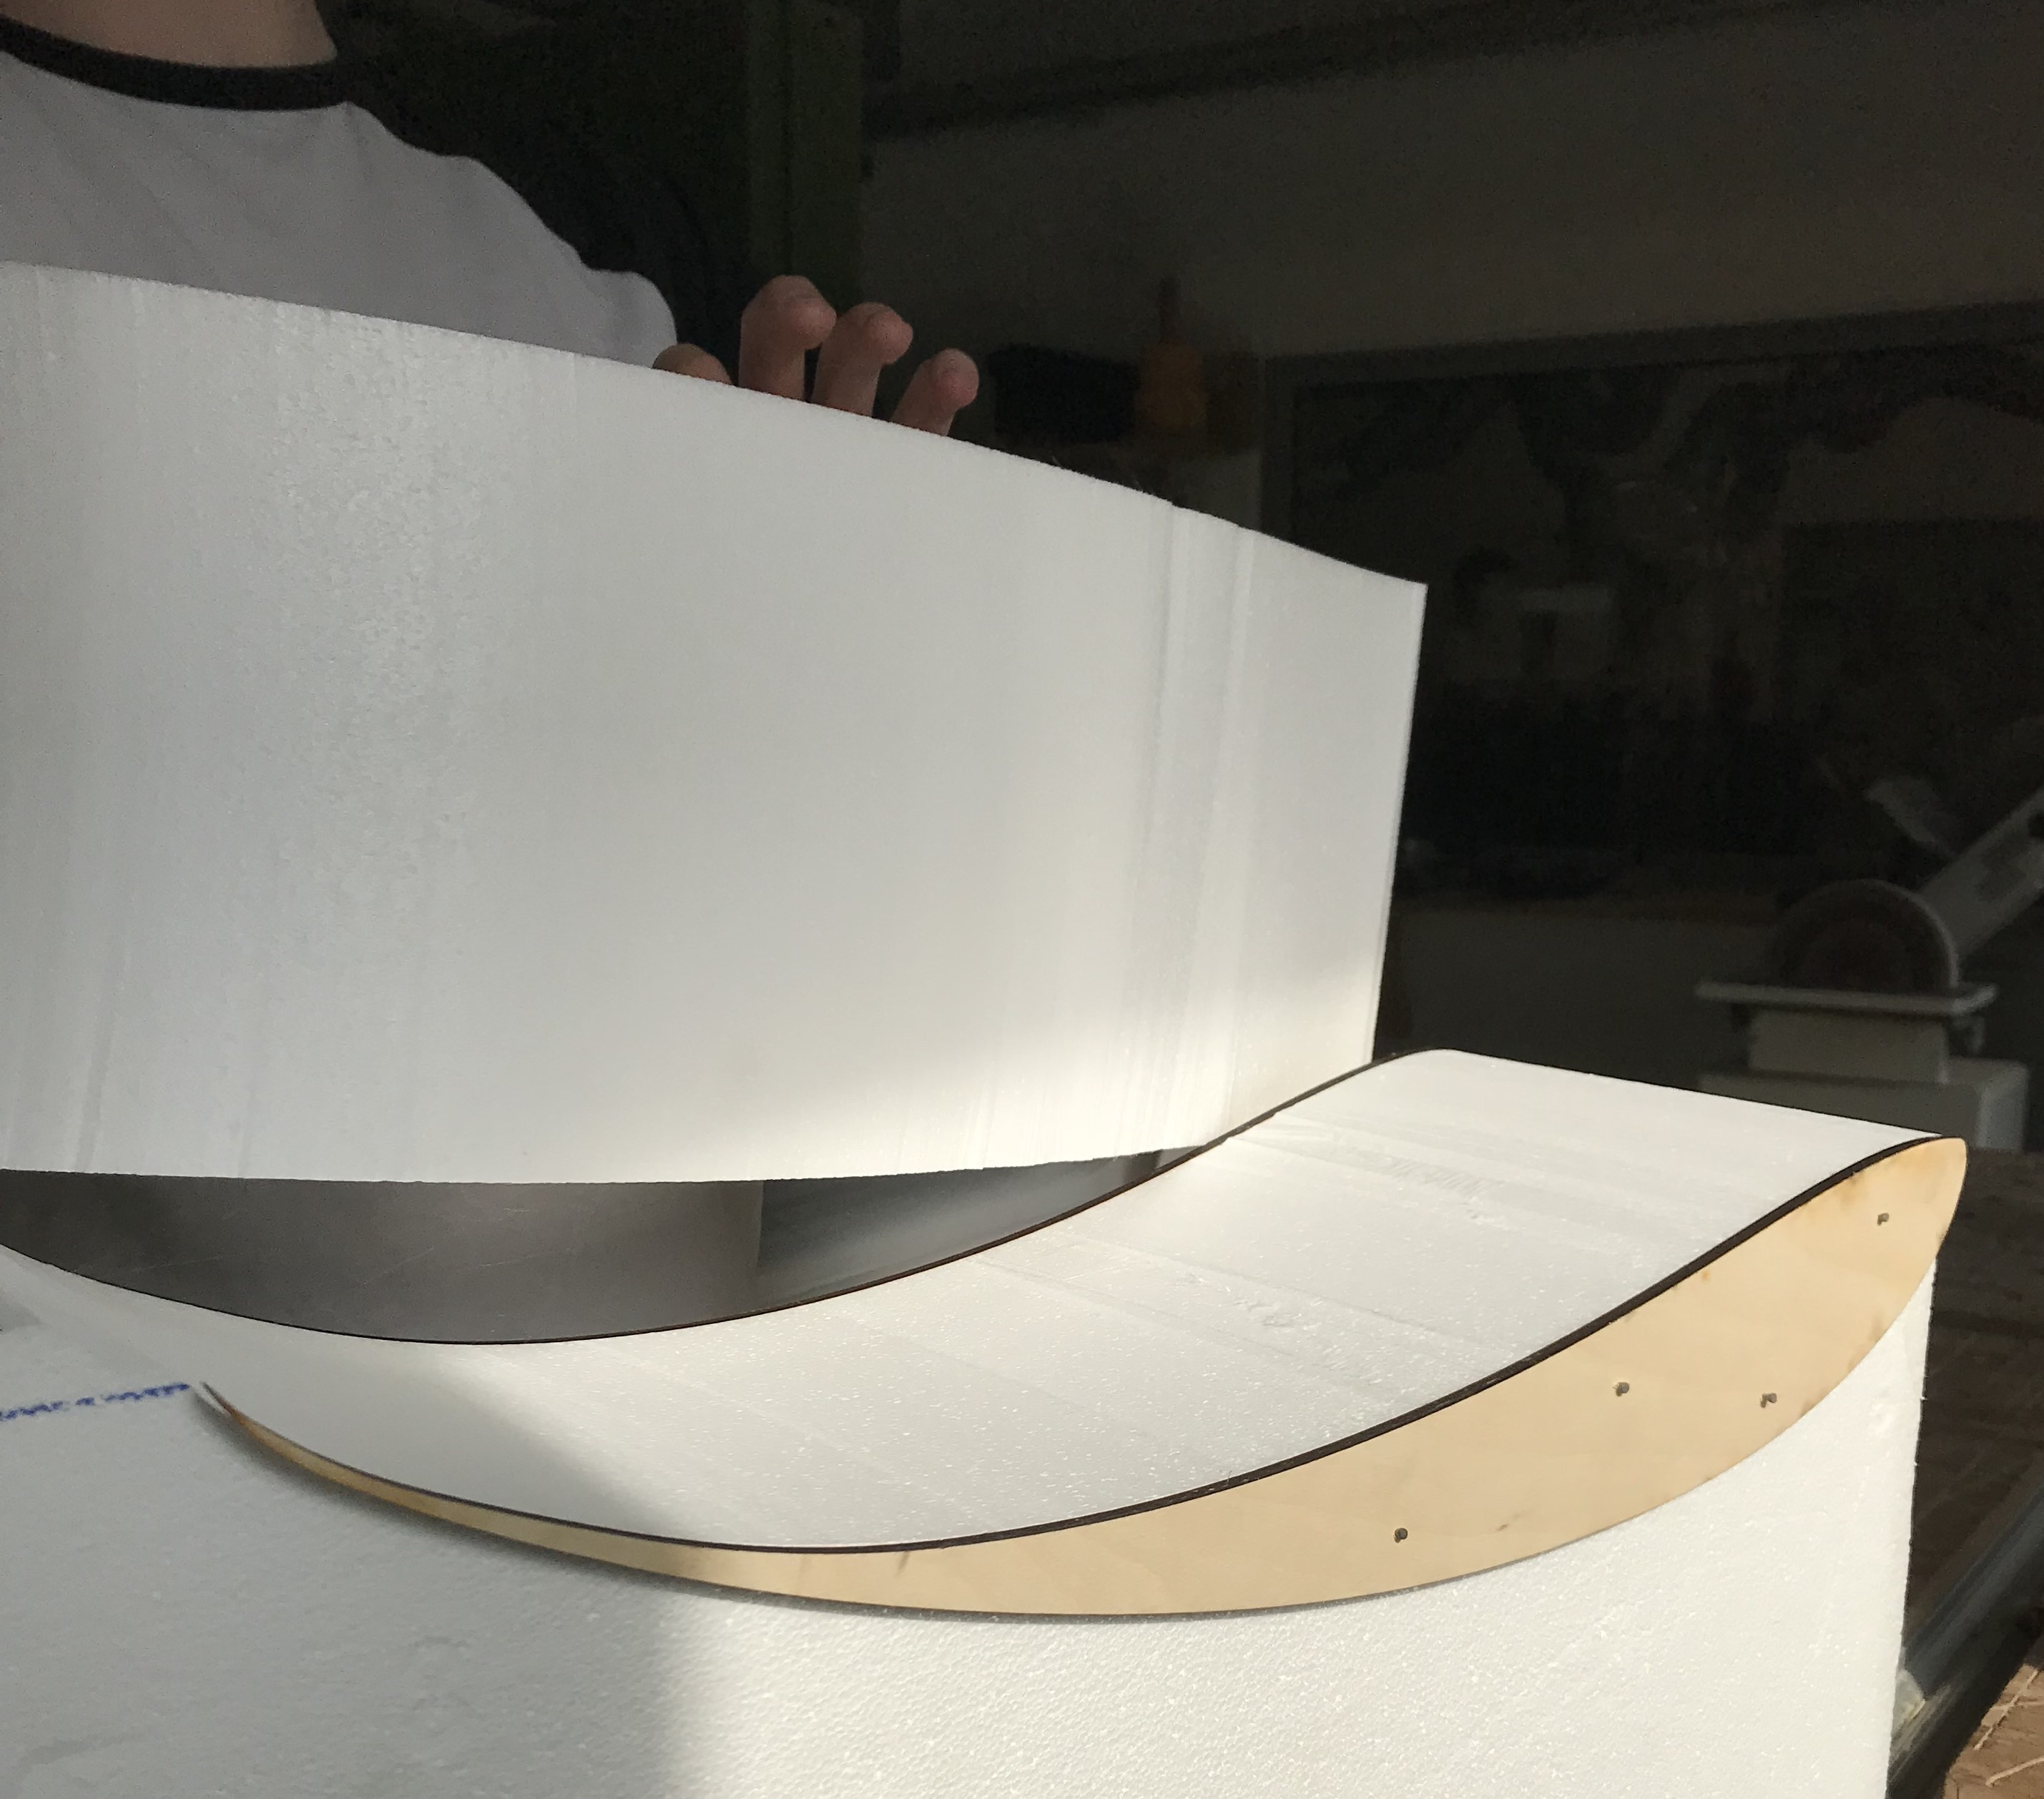
\includegraphics[width=\textwidth]{hotwiredhalf.jpg}
    \caption{Frontal area of the car with a dummy wing inserted into the CAD model, in order to get an estimate of the drag coefficient $C_D$.}
    \label{fig:frontarea}
  \end{figure}

  \begin{align}
    \dot{x}_\text{max} &= \left(\frac{2\cdot \SI{80}{\kilo\watt}}{0.85\left(\SI{1.225}{\kilogram\per\cubic\metre}~ \SI{1.2}{\square\metre}\right)}\right)^{\frac{1}{3}} = \SI{50}{\metre\per\second} = \SI{181.4}{\kilo\metre\per\hour}
    \intertext{however, given the ruleset a forecasted maximum of $\SI{110}{\kilo\metre\per\hour}$ allows a much larger drag coefficient $C_D$:}
    C_D &= \frac{2 P}{\dot{x}^3 \left(\rho A \right)}
    = \frac{2 \cdot \SI{80}{\kilo\watt}}{(\SI{120}{\kilo\metre\per\hour})^3 \left(\SI{1.225}{\kilogram\per\cubic\metre}~ \SI{1.2}{\square\metre} \right)} = 2.82
  \end{align}
  Thus, the car's top speed will only be limited by a drag factor $>2.82$, which is far above the drag introduced by the aerodynamic devices.

  From this derivation, it is clear that the car's abilities at maximum speeds far exceed the requirement of the track. Therefore, the next step is to improve cornering speeds which depend strongly on the tyre's grip on the surface of the road \cite{jkatz}.

\subsection{Downforce Effects on Cornering}
\subsection{Load Distribution}

%Check https://uta-ir.tdl.org/uta-ir/bitstream/handle/10106/24176/Merkel_uta_2502M_%2012503.pdf?sequence=1
